\documentclass{beamer}

\usepackage[scale=2]{ccicons}
\usepackage{stmaryrd}
\usepackage{graphicx}

% Beamer configuration
\usetheme[sectionpage=progressbar, numbering=counter, progressbar=frametitle]{metropolis}

\usepackage{pgfplots}
\usepackage{pgfplotsthemetol}

% Progressbar
\setbeamercolor{progress bar}{
    fg=TolLightGreen,
    bg=TolLightGreen!50!black!30
}
\makeatletter
    \setlength{\metropolis@titleseparator@linewidth}{2pt}
    \setlength{\metropolis@progressonsectionpage@linewidth}{2pt}
    \setlength{\metropolis@progressinheadfoot@linewidth}{2pt}
\makeatother

% Footer
\setbeamertemplate{frame footer}{Quentin Brateau, ENSTA Bretagne}

% Block fill
\metroset{block=fill}

\title{Sea route monitoring by weather buoys using interval analysis}
\date{\today}
\author{Quentin Brateau}
\institute{ENSTA Bretagne}

\begin{document}

    \maketitle

    \section{Introduction}

        \begin{frame}{Introduction}
            \begin{minipage}{0.55\textwidth}
                \begin{block}<1->{Problem statement}
                    Estimate the state of multiples sub-systems governed by the same evolution equation.
                \end{block}
                \begin{block}<2->{Measurements}
                    Sub-systems are sensed by \alert{independant} and \alert{passive} sensors. The number of sensors can be significant.
                \end{block}
            \end{minipage}
            \hfill
            \onslide<3->
            \begin{minipage}{0.4\textwidth}
                \begin{figure}
                    \includegraphics[width=\textwidth]{build/imgs/introduction.pdf}
                    \caption{Multiple systems sensed by multiples sensors}
                \end{figure}
            \end{minipage}
        \end{frame}

    \section{Formalism}

        \begin{frame}{State eqaution}
            \begin{block}<1->{Evolution equation}
                $\forall n \in \mathbb{N}$ the number of systems, $\forall i \in \llbracket 1, n\rrbracket$, $x_i$ is the state of the $i^{th}$ system such that
                \begin{equation}
                    \dot{x_i} = f(x_i)
                \end{equation}
            \end{block}

            \begin{block}<2->{Measurement equation}
                $\forall m \in \mathbb{N}$ the number of sensors, $\forall k \in \llbracket 1, m\rrbracket$, $\exists j \in \llbracket 1, n\rrbracket$ such that
                \begin{equation}
                    g^k(x_i(t_j)) \in \mathbb{Y}_j^k
                \end{equation}
            \end{block}
        \end{frame}

        \begin{frame}{Detection space}
            \begin{block}<1->{Sensor detection set}
                $\forall k \in \llbracket 1, m\rrbracket$, $\mathbb{Y}^k$ is the detection set of the $k^{th}$ sensor such that
                \begin{equation}
                    \mathbb{Y}^k = \bigcup_{j \in \llbracket 1, m\rrbracket} \mathbb{Y}_j^k
                \end{equation}
            \end{block}
            \begin{block}<2->{Detection space}
                $\mathbb{Y} \in \mathbb{R}^k$ is the detection set of all the systems such that
                \begin{equation}
                    \mathbb{Y} = \mathbb{Y}^1 \times \dots \times \mathbb{Y}^m
                \end{equation}
            \end{block}
        \end{frame}

        \begin{frame}{Example}
            \begin{exampleblock}<1->{Example}
                Assuming that $n = 3$, $m = 2$, and
                $$\forall k \in \llbracket 1, m\rrbracket, \;  \forall j \in \llbracket 1, m\rrbracket, \quad \mathbb{Y}_k^j \in \mathbb{R}$$
            \end{exampleblock}
            \begin{exampleblock}<2->{Detection space}
                Then $\mathbb{Y} \in \mathbb{R}^2$ and
                \begin{eqnarray}
                    \mathbb{Y} & = & \mathbb{Y}^1 \times \mathbb{Y}^2 \\
                    & = & \left(\mathbb{Y}_1^1 \cup \mathbb{Y}_2^1 \cup \mathbb{Y}_3^1\right) \times \left(\mathbb{Y}_1^1 \cup \mathbb{Y}_2^1 \cup \mathbb{Y}_3^1\right)
                \end{eqnarray}
            \end{exampleblock}
        \end{frame}

        \begin{frame}{Example}
            \begin{figure}
                \includegraphics[height=0.7\textheight]{example-image-a}
                \caption{Detection space}
            \end{figure}
        \end{frame}

    \section{Application: Sea route monitoring}

        \begin{frame}{Boat wake}
            
        \end{frame}

    \section{Conclusion}
\end{document}